\documentclass{beamer}
\usepackage{graphicx}
\usepackage{amsmath,amssymb,amstext,amsthm,xargs}
\usepackage{amsfonts}
\usepackage{bbm}
\usepackage{beamerthemesplit}

\usepackage[utf8]{inputenc}
\usepackage[french]{babel}
\usepackage{bbm}

\usetheme{Antibes}
\mode<presentation>
\useoutertheme{tree}
\usecolortheme{beaver}
\useinnertheme{rectangles}

\setbeamerfont{block title}{size={}}
%\usecolortheme[rgb={0.55,0.1,0.05}]{structure}
%\usecolortheme[rgb={0.75,0.1,0.05}]{structure}
\usepackage{color}

\newenvironment{disarray}{\everymath{\displaystyle\everymath{}}\array} {\endarray}
\newtheorem{theo}{Théorème}
\newtheorem{prop}[theo]{Proposition}
\newtheorem{conj}[theo]{Conjecture}
\newtheorem{cor}{Corollary}[theo]

\newtheorem{lem}{Lemme}
\newtheorem{nota}{Notation}
\newtheorem{rk}{Remark}
\newtheorem{exa}{Example}
\newtheorem{df}{Definition}
\newtheorem{terminologie}{Terminologie}
\def\rme{\mathrm{e}}
\def\rmi{\mathrm{i}}
\def\rset{\mathbb{R}}
\def\nset{\mathbb{N}}
\def\dlim{\stackrel{d}{\rightarrow}}
\newcommandx{\plim}[1][1=]{\stackrel{\PP_{#1}}{\longrightarrow}}
\def\iid{i.i.d.}
\def\1{\mathbbm{1}}
\newenvironment{dem}{\textbf{Proof}}{\flushright$\blacksquare$\\}
%\def\blankframe{
%\mode<presentation>{
%  { \setbeamertemplate{background canvas}[default]
%    \setbeamercolor{background canvas}{bg=black}
%    \begin{frame}[plain]{}
%    \end{frame}
%  }
%}
%\mode<presentation>{
%\setbeamertemplate{background canvas}[default]
%\setbeamercolor{background canvas}{bg=white}}
%\mode*
%}
\def\eqsp{\,}
\DeclareMathOperator{\E}{{\mathbb E}}
\def\PE{\E}
\def\PCov{\mathrm{Cov}}
\DeclareMathOperator{\F}{{\mathbb F}}
\DeclareMathOperator{\G}{{\mathbb G}}
\DeclareMathOperator{\D}{{\mathbb D}}
\DeclareMathOperator{\R}{{\mathbb R}}
\DeclareMathOperator{\C}{{\mathbb C}}
\DeclareMathOperator{\Z}{{\mathbb Z}}
\DeclareMathOperator{\N}{{\mathbb N}}
\DeclareMathOperator{\K}{{\mathbb K}}
\DeclareMathOperator{\T}{{\mathbb T}}
\DeclareMathOperator{\PP}{{\mathbb P}}
\DeclareMathOperator{\QQ}{{\mathbb Q}}
\DeclareMathOperator{\Q}{{\mathbb Q}}
\DeclareMathOperator{\IF}{{\mathbb I}}


%%%%%%%%%%%%%%%%%%%%%%%%%%%%%%% Pour le modèle lin\'eaire

\DeclareMathOperator{\bX}{\boldsymbol{X}}
\DeclareMathOperator{\bY}{\boldsymbol{Y}}
\DeclareMathOperator{\bx}{\boldsymbol{x}}
\DeclareMathOperator{\vp}{\boldsymbol{p}}
\DeclareMathOperator{\vq}{\boldsymbol{q}}
\DeclareMathOperator{\estMCNL}{\widehat \theta_n^{\,\,{\tt mcnl}}}
\DeclareMathOperator{\estMV}{\widehat \theta_n^{\,\,{\tt mv}}}
\DeclareMathOperator{\est}{\widehat \theta_{\mathnormal{n}}}
\DeclareMathOperator{\var}{\mathrm{Var}}
\def\Var{\var}
\DeclareMathOperator{\estMVc}{\widehat \theta_{n,0}^{\,{\tt mv}}}
\DeclareMathOperator{\Xbar}{\overline{\mathnormal{X}}_\mathnormal{n}}

\newcommand{\indi}[1]{\mathbbm{1}_{\{#1\}}}
\newcommand{\coint}[1]{\left[#1\right)}
\newcommand{\ocint}[1]{\left(#1\right]}
\newcommand{\ooint}[1]{\left(#1\right)}
\newcommand{\ccint}[1]{\left[#1\right]}

\definecolor{LightYell}{rgb}{0.95,0.83,0.70}
\definecolor{orange}{rgb}{1.0,0.50,0.01}
\definecolor{StroYell}{rgb}{0.95,0.88,0.72}
\definecolor{lightred}{rgb}{0.75,0.033,0}
\definecolor{shadecolor1}{rgb}{0.90,0.83,0.70}
\definecolor{myem}{rgb}{0.797,0.598,0.598}
\definecolor{BrickRed}{cmyk}{0,0.89,0.94,0.28}
\definecolor{RoyalPurple}{cmyk}{0.75,0.9,0,0}

\newcommand{\tco}[1]{\textcolor{orange}{#1}}
\newcommand{\tcr}[1]{\textcolor{lightred}{#1}}

\def\gauss{\mathcal{N}}
\def\truetheta{\theta}
\def\truebeta{\boldsymbol{\beta}}
\def\projX{A}
\def\curtheta{\alpha}
\def\argmin{\mathrm{argmin}}
\def\ie{\emph{i.e.}}
\def\regressmat{\mathbb{X}}
\def\errpred{\boldsymbol{\hat{\xi}}}
\def\bnoise{\boldsymbol{\xi}}
\def\predY{\hat{\mathbf{Y}}}
\DeclareMathOperator{\estregress}{\widehat{\truebeta}_n}
\DeclareMathOperator{\estMC}{\widehat \theta_n^{\,\,{\tt mc}}}
\def\curbeta{b}
\def\bcurbeta{\mathbf{b}}
\newcommand{\indep}{\rotatebox[origin=c]{90}{$\models$}} 
\newcommand{\Id}[1]{\mathrm{Id}_{#1}}
\title{MAP 433 : Introduction aux méthodes statistiques. Cours 3}
%\author{M. Hoffmann}
%\institute{Université Paris-Est and ETG}
\begin{document}
\date{11 Septembre 2015}
\maketitle



\begin{frame}
\frametitle{Aujourd'hui}
\tableofcontents
\end{frame}
\section{Modélisation statistique}
\subsection{Expérience statistique}
\begin{frame}
\frametitle{Expérience statistique} Consiste à identifier:
\begin{itemize}
\item \alert{Des observations}
$${\tt x}_1,{\tt x}_2,\ldots, {\tt x}_n$$
\alert{considérées} comme des \alert{ réalisations} de variables aléatoires $Z = (X_1,\ldots, X_n)$ de loi $\PP^Z$.
\item \alert{Une famille de lois}
$$\left\{\PP_\theta,\,\theta \in \Theta\right\}.$$
\item \alert{Une problématique} : retrouver le paramètre
$\theta$ tel que $\PP^Z=\PP_\theta$ (estimation) ou bien prendre une décision sur une propriété relative à $\theta$ (test).
\end{itemize}
\end{frame}

\begin{frame}
\frametitle{Expérience statistique}
\begin{itemize}
\item Approche param\'etrique: \alert{ on suppose} que $F$ appartient \`a une
\alert{ famille de lois connue} index\'ee par un param\`etre
$\theta$ de dimension finie: $\theta\in \Theta \subset \R^d$.
\begin{itemize}
\item \underline{Exemple}: $\Theta = \R$,
$$ X_i= \theta +\xi_i, \quad i=1,\dots,n,$$
$\xi_i$ v.a. i.i.d. de densit\'e \alert{ connue} $f$ sur $\R$
et $\E(X_i)=\theta$.

\underline{Question}: en utilisant cette information
suppl\'ementaire, peut-on construire un estimateur plus performant
que l'estimateur $\bar X_n$ bas\'e sur l'approche empirique?
\end{itemize}
%
\end{itemize}
\end{frame}


\begin{frame}
\frametitle{Expérience statistique}
\begin{itemize}
\item En \'ecrivant
$$ X_i= \theta +\xi_i, \quad i=1,\dots,n,$$
$\xi_i$ v.a. i.i.d. de densit\'e \alert{ connue} $f$, nous
pr\'ecisons la forme de la loi $\PP_{\theta}$ de
$(X_1,\dots,X_n)$:
$$\PP_\theta\big[A\big] = \int_A
\left(\prod_{i=1}^n f(x_i-\theta)\right) dx_1\ldots dx_n,
$$
pour tout $A\in {\mathcal B}(\R^n)$.
\end{itemize}
\end{frame}


\begin{frame}
\frametitle{Expérience statistique}
\begin{df}
Une expérience (un modèle) statistique ${\mathcal E}$ est le triplet
$${\mathcal E} = \left(\mathfrak{Z}, {\mathcal Z}, \,\big\{\PP_\theta, \theta \in \Theta\big\}\right),$$
avec
\begin{itemize}
\item $\big(\mathfrak{Z}, {\mathcal Z}\big)$ espace mesurable (souvent
$(\R^n,{\mathcal B}(\R^n))$),
\item $\{\PP_\theta,\,\theta \in \Theta\}$ famille de probabilités définies \alert{simultanément} sur le même espace  $\big(\mathfrak{Z}, {\mathcal Z}\big)$,
\item $\theta$ est le \alert{paramètre inconnu}, et $\Theta$ est \alert{ l'ensemble des paramètres connu}.
\end{itemize}
\end{df}
\end{frame}


%\begin{frame}
%\frametitle{Description (mathématique) d'une expérience statistique}
%\begin{itemize}
%\item Deux points de vue \alert{ équivalents} et (parfois ?) source de confusion :
%\begin{itemize}
%\item Expérience \underline{engendrée par une observation}.
%\item Expérience \underline{canonique}
%\end{itemize}
%\item \alert{Traitement sur un exemple} : on  observe  $X_1,\ldots, X_n$ i.i.d. de loi exponentielle de paramètre $\theta >0$.
%\end{itemize}
%\end{frame}


\begin{frame}
\frametitle{Experience engendrée par ($X_1,\ldots, X_n$)}
\begin{itemize}
\item \alert{Traitement sur un exemple} : on observe
$$Z = (X_1,\ldots, X_n), \quad\quad X_i= \theta + \xi_i,$$
$\xi_i$ v.a. i.i.d. de densit\'e \alert{ connue} $f$.
\item La famille de lois $\big\{\PP_\theta^n,\theta \in \Theta  =
\R\big\}$ est définie sur $\mathfrak{Z}=\R^n$ par
$$\PP_\theta^n\big[A\big] = \int_A
\left(\prod_{i=1}^n f(x_i-\theta)\right) dx_1\ldots dx_n,
$$
pour $A\in{\mathcal Z}= {\mathcal B}(\R^n)$ (et $\PP^Z$ est l'une
des $\PP_\theta^n$).
\item Expérience \alert{engendrée par l'observation $Z$} :
$${\mathcal E}^n = \big(\R^n,{\mathcal B}(\R^n),\big\{\PP_\theta^n,\,\theta \in \Theta\big\}\big).$$
\end{itemize}
\end{frame}

%\begin{frame}
%\frametitle{Expérience -- observation canonique}
%\begin{itemize}
%\item Si on part de ${\mathcal E}^n = \big(\R^n,{\mathcal B}(\R^n),\big\{\PP_\theta^n,\,\theta \in \Theta\big\}\big)$, \alert{il n'y a plus d'observation !} On a perdu la structure (trop lourde) de tout l'espace $\big(\Omega, {\mathcal F}, \PP\big)$ et des observations $X_1,\ldots, X_n$.
%\item On peut \alert{toujours  fabriquer  une observation} $Z$ dont l'expérience engendrée soit ${\mathcal E}^n$.
%Il suffit de poser
%$$\big(\Omega, {\mathcal F}\big):=\big(\mathfrak{Z}, {\mathcal Z}\big) \stackrel{\text{ici}}{=}\big(\R^n,{\mathcal B}(\R^n)\big),$$
%et
%$$Z(\omega) = \omega\;\;\;\text{observation canonique}.$$
%\end{itemize}
%\end{frame}

\begin{frame}
\frametitle{Expérience (mod\`ele) paramétrique, non-paramétrique}
\begin{itemize}
\item Si $\Theta$ peut être  pris  comme un sous-ensemble
de $\R^d$ : \alert{ expérience (=mod\`ele) paramétrique}.
\item Sinon (par exemple si le paramètre $\theta$ est un élément d'un espace fonctionnel) : \alert{ expérience (=mod\`ele) non-paramétrique}.
\end{itemize}
\end{frame}

\subsection{Expériences dominées}
\begin{frame}
\frametitle{Expériences dominées}
\begin{itemize}
\item On fait une hypothèse minimale de  complexité  sur le modèle statistique. \alert{ But} : ramener l'étude de la famille
$$\{\PP_\theta,\,\theta \in \Theta\}$$
à l'étude d'une famille de fonctions
$$\left\{z \in \mathfrak{Z} \leadsto f(\theta,z) \in \R_+,\,\theta \in \Theta\right\}.$$
\item Via la notion de \alert{ domination}. Si $\mu,\nu$ sont deux mesures $\sigma$-finies sur $\mathfrak{Z}$, alors $\mu$ \alert{ domine} $\nu$ (notation $\nu \ll \mu$) si
$$\mu\big[A\big]=0 \Rightarrow \nu\big[A\big]=0.$$
\end{itemize}
\end{frame}
\begin{frame}
\frametitle{Théorème de Radon-Nikodym}
\begin{theo}
Si $\nu \ll \mu$, il existe une fonction positive
$$z \leadsto  p(z) \stackrel{\text{notation}}{=} \frac{d\nu}{d\mu}(z),$$ définie $\mu-$p.p., $\mu-$ intégrable, telle que
$$\nu\big[A\big] = \int_{A}p(z) \mu(dz) = \int_{A}\tfrac{d\nu}{d\mu}(z)\mu(dz),\;\;A \in {\mathcal Z}.$$
%\underline{Notation} :
%$$p(z)=\frac{d\nu}{d\mu}(z),\;\;\text{densité de}\;\nu\;\text{par rapport à}\;\mu.$$
\end{theo}
\end{frame}
\begin{frame}
\frametitle{Expérience dominée}
\begin{df}
Une expérience statistique ${\mathcal E} = \big(\mathfrak{Z}, {\mathcal Z}, \big\{\PP_\theta, \theta \in \Theta\big\}\big)$ est \alert{dominée} par la mesure $\sigma$-finie $\mu$ définie sur $\mathfrak{Z}$ si
$$\forall \theta \in \Theta : \PP_\theta \ll \mu.$$
\end{df}
On appelle \alert{ densités} de la famille $\{\PP_\theta,\theta \in \Theta\}$ la famille de fonctions (définies $\mu-$ p.p.)
$$z\leadsto \frac{d\PP_\theta}{d\mu}(z),\;z\in \mathfrak{Z},\;\theta \in \Theta.$$
\end{frame}

\begin{frame}
\frametitle{Densité, régression}
Deux classes d'expériences statistiques \alert{dominées} fondamentales :
\begin{itemize}
\item Le modèle de \alert{ densité}
\item Le modèle de \alert{régression }
\end{itemize}
\end{frame}


\subsection{Modèle de densité}

\begin{frame}
\frametitle{Modèle de densité (paramétrique)}
\begin{itemize}
\item On observe un $n$-échantillon de v.a.r. $X_1,\ldots, X_n$.
\item La loi des $X_i$ appartient à
$\{\PP_\theta,\,\theta \in \Theta\}$, famille de \alert{probabilités sur $\R$}, \alert{ dominée} par une mesure ($\sigma$-finie) $\mu(dx)$ sur $\R$.
\item La loi de $(X_1,\ldots,X_n)$ s'écrit
\begin{align*}
\PP_\theta^n(dx_1\cdots dx_n) & = \PP_\theta(dx_1)\otimes \cdots \otimes \PP_\theta(dx_n) \\
& \ll  \mu(dx_1)\otimes \cdots \otimes \mu(dx_n) \\
& \stackrel{\text{\alert{notation}}}{=} \mu^n(dx_1\cdots dx_n)
\end{align*}
%\item \alert{L'expérience statistique} engendrée par $(X_1,\ldots, X_n)$ s'écrit :
%$${\mathcal E}^n = \Big(\R^n, {\mathcal B}(\R^n), \big\{\PP_\theta^n,\theta \in \Theta\big\}\Big),\;\;\alert{\Theta \subset \R^d}.$$
\end{itemize}
\end{frame}

\begin{frame}
\frametitle{Modèle de densité (paramétrique)}
\begin{itemize}
\item \alert{ Densité du modèle} : on part de
$$f(\theta,x)=\frac{d\PP_\theta}{d\mu}(x),\;\;x\in \R$$
et
$$\frac{d\PP_\theta^n}{d\mu^{n}}(x_1,\ldots, x_n) = \prod_{i = 1}^n f(\theta,x_i),\;\;x_1,\ldots, X_n \in \R.$$
\item  \alert{L'expérience statistique} engendrée par $(X_1,\ldots, X_n)$ s'écrit :
$${\mathcal E}^n = \Big(\R^n, {\mathcal B}(\R^n), \big\{\PP_\theta^n,\theta \in \Theta\big\}\Big),\;\;\alert{\Theta \subset \R^d}.$$
\end{itemize}
\end{frame}

\begin{frame}
\frametitle{Exemple 1 : modèle de densité gaussienne univariée}
\begin{itemize}
\item $X_i\sim {\mathcal N}(m,\sigma^2)$,
avec
$$\theta = (m,\sigma^2) \in \Theta = \R\times \R_+\setminus\{0\}.$$
\begin{align*}
\PP_\theta(dx) = f(\theta,x)dx & =\frac{1}{\sqrt{2\pi \sigma^2}}\exp\Big(-\frac{(x-m)^2}{2\sigma^2}\Big)dx \\
& \ll \mu(dx)=dx.
\end{align*}
\item Puis
\begin{align*}
\frac{d\PP_{\alert{\theta}}^n}{d\mu^n}(x_1,\ldots, x_n) & = \prod_{i = 1}^n f(\alert{\theta},x_i) \\
& =(2\pi \alert{\sigma^2})^{-n/2}\exp\big(-\frac{1}{2\alert{\sigma^2}}\sum_{i = 1}^n (x_i-\alert{m})^2\big),
\end{align*}
avec $x_1,\ldots,x_n \in \R$.
\end{itemize}
\end{frame}

\begin{frame}
\frametitle{Exemple 2 :  modèle de Bernoulli}
\begin{itemize}
\item $X_i \sim \text{Bernoulli}(\theta)$, avec $\theta \in \Theta = [0,1]$.
\begin{align*}
\PP_\theta(dx)& = (1-\theta)\, \delta_{0}(dx) + \theta\, \delta_1(dx) \\
& \ll \mu(dx) = \delta_0(dx)+\delta_1(dx)\;\;\text{(mesure de comptage)}.
\end{align*}
\item Puis
$$\boxed{\frac{d\PP_{\tco{\theta}}}{d\mu}(x) = (1-\tco{\theta})\,\1_{\{x=0\}}+\tco{\theta}\,\1_{\{x=1\}} = \tco{\theta}^x(1-\tco{\theta})^{1-x}}
$$
\alert{avec $x\in \{0,1\}$} (et $0$ sinon), et
$$\frac{d\PP_\theta^n}{d\mu^n}(x_1\cdots x_n) = \prod_{i = 1}^n \theta^{x_i}(1-\theta)^{1-x_i},$$
\alert{avec $x_i \in \{0,1\}$} (et $0$ sinon).
\end{itemize}
\end{frame}

\begin{frame}
\frametitle{Exemple 3 : temps de panne  arrêtés}
\begin{itemize}
\item On observe $X_1,\ldots, X_n$, où $X_i = Y_i \wedge T$, avec $Y_i$ \alert{lois exponentielles} de paramètre $\theta$ et $T$ \alert{temps fixe} (censure).
\item Cas 1 : $T=\infty$ (pas de censure). Alors  $\theta \in \Theta = \R_+\setminus \{0\}$ et
$$\PP_\theta(dx) = \theta \exp(-\theta x)1_{\{x \geq 0\}}dx \ll \mu(dx) = dx$$
et
$$\frac{d\PP_{\tco{\theta}}^n}{d\mu^n}(x_1,\ldots,x_n) = \alert{\theta}^n \exp\Big(-\alert{\theta} \sum_{i = 1}^n x_i\Big),$$
\alert{avec $x_i \in \R_+$} (et $0$ sinon).
\item Cas 2 : \alert{Comment s'écrit le modèle} dans la cas où $T<\infty$ (présence de censure) ? Comment choisir $\mu$ ?
\end{itemize}
\end{frame}




%\subsection{Modèle de régression}
%
%
%
%
%\begin{frame}
%\frametitle{Expérience statistique}
%%\begin{itemize}
%%\item
%Une \alert{expérience (un modèle) statistique} ${\mathcal E}$ est la donnée d'un triplet
%$$\boxed{{\mathcal E} = \left(\mathfrak{Z}, {\mathcal Z}, \,\big\{\PP_\theta, \theta \in \Theta\big\}\right)}$$
%avec
%\begin{itemize}
%\item $\big(\mathfrak{Z}, {\mathcal Z}\big)$ espace d'état (des observables, en général $\R^n$),
%\item $\{\PP_\theta,\,\theta \in \Theta\}$ famille de probabilités définies \alert{simultanément} sur le même espace  $\big(\mathfrak{Z}, {\mathcal Z}\big)$,
%\item $\theta$ \alert{paramètre inconnu}, $\Theta$ \alert{ l'ensemble des paramètres}.
%\end{itemize}
%%\item L'expérience ${\mathcal E}$ est \alert{ dominée} s'il existe une mesure $\sigma$-finie $\mu$ sur $\mathfrak{Z}$ telle que $\PP_\theta \ll \mu$ pour tout $\theta \in \Theta$.
%%\end{itemize}
%\end{frame}
%
%
%\begin{frame}
%\frametitle{Experience engendrée par ($X_1,\ldots, X_n$)}
%\begin{itemize}
%\item \alert{Traitement sur un exemple} : on observe
%$$Z = (X_1,\ldots, X_n), \quad\quad X_i= \theta + \xi_i,$$
%$\xi_i$ v.a. i.i.d. de densit\'e \alert{ connue} $f$.
%\item La famille de lois $\big\{\PP_\theta^n,\theta \in \Theta  =
%\R\big\}$ est définie sur $\mathfrak{Z}=\R^n$ par
%$$\PP_\theta^n\big[A\big] = \int_A
%\left(\prod_{i=1}^n f(x_i-\theta)\right) dx_1\ldots dx_n,
%$$
%pour $A\in{\mathcal Z}= {\mathcal B}(\R^n)$ (et $\PP^Z$ est l'une
%des $\PP_\theta^n$).
%\item Expérience \alert{engendrée par l'observation $Z$} :
%$${\mathcal E}^n = \big(\R^n,{\mathcal B}(\R^n),\big\{\PP_\theta^n,\,\theta \in \Theta\big\}\big).$$
%\end{itemize}
%\end{frame}
%
%
%\begin{frame}
%\frametitle{Expérience (mod\`ele) paramétrique, non-paramétrique}
%\begin{itemize}
%\item Si $\Theta$ peut être  pris  comme un sous-ensemble
%de $\R^d$ : \alert{ expérience (=mod\`ele) paramétrique}.
%\item Sinon (par exemple si le paramètre $\theta$ est un élément d'un espace fonctionnel) : \alert{ expérience (=mod\`ele) non-paramétrique}.
%\end{itemize}
%\end{frame}
%
%\subsection{Expériences dominées}
%\begin{frame}
%\frametitle{Expériences dominées}
%\begin{itemize}
%\item On fait une hypothèse minimale de  complexité  sur le modèle statistique. \alert{ But} : ramener l'étude de la famille
%$$\{\PP_\theta,\,\theta \in \Theta\}$$
%à l'étude d'une famille de fonctions
%$$\left\{z \in \mathfrak{Z} \leadsto f(\theta,z) \in \R_+,\,\theta \in \Theta\right\}.$$
%\item Via la notion de \alert{ domination}. Si $\mu,\nu$ sont deux mesures $\sigma$-finies sur $\mathfrak{Z}$, alors $\mu$ \alert{ domine} $\nu$ (notation $\nu \ll \mu$) si
%$$\mu\big[A\big]=0 \Rightarrow \nu\big[A\big]=0.$$
%\end{itemize}
%\end{frame}
%\begin{frame}
%\frametitle{Théorème de Radon-Nikodym}
%\begin{theo}
%Si $\nu \ll \mu$, il existe une fonction positive
%$$z \leadsto  p(z) \stackrel{\text{notation}}{=} \frac{d\nu}{d\mu}(z),$$ définie $\mu-$p.p., $\mu-$ intégrable, telle que
%$$\nu\big[A\big] = \int_{A}p(z) \mu(dz) = \int_{A}\tfrac{d\nu}{d\mu}(z)\mu(dz),\;\;A \in {\mathcal Z}.$$
%%\underline{Notation} :
%%$$p(z)=\frac{d\nu}{d\mu}(z),\;\;\text{densité de}\;\nu\;\text{par rapport à}\;\mu.$$
%\end{theo}
%\end{frame}
%\begin{frame}
%\frametitle{Expérience dominée}
%\begin{df}
%Une expérience statistique ${\mathcal E} = \big(\mathfrak{Z}, {\mathcal Z}, \big\{\PP_\theta, \theta \in \Theta\big\}\big)$ est \alert{dominée} par la mesure $\sigma$-finie $\mu$ définie sur $\mathfrak{Z}$ si
%$$\forall \theta \in \Theta : \PP_\theta \ll \mu.$$
%\end{df}
%On appelle \alert{ densités} de la famille $\{\PP_\theta,\theta \in \Theta\}$ la famille de fonctions (définies $\mu-$ p.p.)
%$$z\leadsto \frac{d\PP_\theta}{d\mu}(z),\;z\in \mathfrak{Z},\;\theta \in \Theta.$$
%\end{frame}
%
%\begin{frame}
%\frametitle{Densité, régression}
%Deux classes d'expériences statistiques \alert{dominées} fondamentales :
%\begin{itemize}
%\item Le modèle de \alert{ densité} (Cours 3)
%\item Le modèle de \alert{régression } (Cours 4)
%\end{itemize}
%\end{frame}
%
%
%\begin{frame}
%\frametitle{Modèle de densité paramétrique}
%\begin{itemize}
%\item On observe un $n$-échantillon de v.a.r. $X_1,\ldots, X_n$.
%\item La loi des $X_i$ appartient à
%$\{\PP_\theta,\,\theta \in \Theta\}$, famille de \alert{probabilités sur $\R$}, indicée par $\Theta \subset \R^d$, \alert{ dominée} par une mesure ($\sigma$-finie) $\mu(dx)$ sur $\R$.
%\item Loi de $(X_1,\ldots,X_n)$
%$$
%\boxed{\PP_\theta^n(dx_1\cdots dx_n)  =\prod_{i=1}^n f(\theta, x_i)\mu^n(dx_1\ldots dx_n)}$$
%avec
%$$ f(\theta,x) = \frac{d\PP_\theta}{d\mu}(x)$$
%et $\mu^n(dx_1\ldots dx_n) =\mu(dx_1)\otimes \ldots \otimes \mu(dx_n)$.
%\end{itemize}
%\end{frame}
%
%
%\begin{frame}
%\frametitle{Exemple : modèle de Bernoulli}
%\begin{itemize}
%\item $X_i \sim \text{Bernoulli}(\theta)$, avec $\theta \in \Theta = [0,1]$.
%\begin{align*}
%\PP_\theta(dx)& = (1-\theta)\, \delta_{0}(dx) + \theta\, \delta_1(dx)\\
%& \ll \mu(dx) = \delta_0(dx)+\delta_1(dx).
%\end{align*}
%\item Puis
%$$\boxed{\frac{d\PP_{\tco{\theta}}}{d\mu}(x) = (1-\alert{\theta})\,1_{\{x=0\}}+\alert{\theta}\,1_{\{x=1\}} = \alert{\theta}^x(1-\alert{\theta})^{1-x}}$$
%\alert{avec $x\in \{0,1\}$} (et $0$ sinon), et
%\begin{align*}
%\frac{d\PP_\theta^n}{d\mu^n}(x_1,\cdots, x_n) & = \prod_{i = 1}^n \theta^{x_i}(1-\theta)^{1-x_i} \\
%& =\theta^{\sum_{i = 1}^n x_i}(1-\theta)^{n-\sum_{i = 1}^nx_i}.
%\end{align*}
%%\alert{avec $x_i \in \{0,1\}$} (et $0$ sinon).
%\item Remarque : choix des \alert{ espaces...}
%\end{itemize}
%\end{frame}
%
%\begin{frame}
%\frametitle{Exemple : temps de panne  arrêtés}
%\begin{itemize}
%\item On observe $X_1,\ldots, X_n$, où $X_i = Y_i \wedge T$, avec $Y_i$ \alert{lois exponentielles} de paramètre $\theta$ et $T$ \alert{temps fixe} (censure).
%\item Cas 1 : $T=\infty$ (pas de censure). Alors  $\theta \in \Theta = \R_+\setminus \{0\}$ et
%$$\PP_\theta(dx) = \theta \exp(-\theta x)1_{\{x \geq 0\}}dx \ll \mu(dx) = dx$$
%et
%$$\frac{d\PP_{\tco{\theta}}^n}{d\mu^n}(x_1,\ldots,x_n) = \alert{\theta}^n \exp\Big(-\alert{\theta} \sum_{i = 1}^n x_i\Big),
%%\prod_{i = 1}^n 1_{x_i \geq 0},
%$$
%\alert{pour $x_i \geq 0$}, et $0$ sinon.
%
%\end{itemize}
%\end{frame}
%
\begin{frame}
\frametitle{Exemple : temps de panne  arrêtés}
\begin{itemize}
%\item Cas 2 : \alert{Comment s'écrit le modèle} dans la cas où $T<\infty$ (présence de censure) ? Comment choisir $\mu$ ?
\item \underline{Loi $\PP_\theta(dx)$ de $X = Y \wedge T$} : $Y \sim$ exponentielle de paramètre $\theta$ :
$$\boxed{X = Y 1_{\{Y < T\}} + T 1_{\{Y \geq T\}}}$$
d'où
\begin{align*}\PP_\theta(dx) &
= \theta e^{-\theta x} 1_{\{0 \leq x < T\}} dx+ \big(\int_{T}^{+\infty}\theta e^{-\theta y}dy\big) \delta_T(dx)\\
&= \theta e^{-\theta x} 1_{\{0 \leq x < T\}}dx + e^{-\theta T} \delta_T(dx) \\
&\ll \mu(dx) = dx + \delta_T(dx)\;\;\; \text{(par exemple)}.
\end{align*}
%(définie $\mu$-pp).
\end{itemize}
\end{frame}

\begin{frame}
\frametitle{Exemple : temps de panne  arrêtés (fin)}
\begin{itemize}
\item Alors, pour ce choix de mesure dominante
$$\boxed{\frac{d\PP_{\tco{\theta}}}{d\mu}(x) = \alert{\theta} e^{-\alert{\theta} x} 1_{\{0 \leq x < T\}} +  e^{-\alert{\theta} T}1_{\{x=T\}}}$$
\item Finalement,
$$\PP_\theta^n(dx_1,\ldots dx_n)
\ll \mu^n(dx_1 \ldots dx_n) = \bigotimes_{i = 1}^n \big[dx_i +
\delta_{T}(dx_i)\big]
$$
et
\begin{align*}
\frac{d\PP_\theta^n}{d\mu^n}(x_1,\ldots, x_n) & = \prod_{i = 1}^n \big(\theta e^{-\theta x_i} 1_{\{0 \leq x_i < T\}} +  e^{-\theta T}1_{\{x_i=T\}}\big) \\
& = \theta^{N_n(T)} e^{-\theta \sum_{i = 1}^{n}x_i 1_{\{x_i<T\}}}e^{-\theta T\big(n-N_n(T)\big)},
\end{align*}
\alert{ avec $0 \leq x_i \leq T$} et $0$ sinon, et  $N_n(T) = \sum_{i = 1}^n1_{\{x_i < T\}}$.
\end{itemize}
\end{frame}




\section{Méthodes d'estimation pour le modèle de densité}


\begin{frame}
\frametitle{Méthodes d'estimation }
\begin{itemize}
%\item Situation
\item Méthode de substitution (ou des moments)
\item $Z$-estimation
\item $M$-estimation
\item Le principe du \alert{ maximum de vraisemblance}
\end{itemize}
\end{frame}

%\begin{frame}
%\frametitle{Situation}
%\end{frame}

\subsection{Méthode des moments}

\begin{frame}
\frametitle{Méthode des moments : dimension 1}
\begin{itemize}
\item $X_1,\ldots, X_n \sim_{\text{i.i.d.}} \PP_\theta$, avec $\theta \in \Theta \;\alert{ \subset \R}$.
\item \underline{Principe} : trouver $g:\R\rightarrow \R$ (en général $g(x)=x^k$) et $h:\R\rightarrow \R$ \alert{ régulières} de sorte que
$$\theta  = h\big(\E_{\alert{\theta}}\big[g(X)\big]\big) = h\Big(\int_{\R}g(x)dF_{\alert{\theta}}(x)\Big)=T(F_{\alert{\theta}})$$
et $T$ fonctionnelle régulière de la distribution inconnnue $F_{\alert{\theta}}$.
\item \underline{Estimateur} :  plug-in
$$\widehat \theta_n = h\big(\tfrac{1}{n}\sum_{i = 1}^n g(X_i)\big).$$
\end{itemize}
\end{frame}

\begin{frame}
\frametitle{Méthode des moments}
\begin{itemize}
\item \underline{Précision d'estimation} via les techniques empiriques :
$$\sqrt{n}\big(\widehat \theta_n - \theta\big) \stackrel{d}{\rightarrow} {\mathcal N}\big(0, h'(\E_{\alert{\theta}}[g(X)])^2\mathrm{Var}_{\alert{ \theta}}[g(X)]\big)$$
en \alert{ loi sous $\PP_\theta$} et la variance asymptotique dépend en général de $\alert{\theta}$ $\rightarrow$ élimination par estimation préliminaire licite via le lemme de Slutsky.
\item \underline{Exemple} : $X_1,\ldots, X_n\sim_{\text{i.i.d.}}$ exponentielle de paramètre $\theta$. On a
$$\E_\theta\big[X\big] = \frac{1}{\theta},$$
l'estimateur par moment associé s'écrit
$$\est = \frac{1}{\overline{X}_n}.$$
\end{itemize}
\end{frame}

\begin{frame}
\frametitle{Exemple en dimension $d>1$}
\begin{itemize}
%\item Le cas de la dimension $d >1$ \alert{sur un exemple} :
\item $X_1,\ldots,X_n \sim_{\text{i.i.d.}}$ Béta$(\alpha,\beta)$, de densité
$$x \leadsto \frac{\Gamma(\alpha+\beta)}{\Gamma(\alpha)\Gamma(\beta)}x^{\alpha-1}(1-x)^{\beta-1}1_{\{0 < x < 1\}},$$
\item Le paramètre est $\alert{\theta} = (\alpha,\beta) \in \alert{\Theta}=\R_+\setminus\{0\} \times \R_+\setminus\{0\}$.
\item On a
$$\boxed{\E_\theta\big[X\big]=\frac{\alpha}{\alpha+\beta},\;\;\E_\theta\big[X^2\big]=\frac{\alpha(\alpha+1)}{(\alpha+\beta+1)(\alpha+\beta)}}$$
\end{itemize}
\end{frame}

\begin{frame}
\frametitle{Exemple en dimension $d>1$}
\begin{itemize}
\item \alert{L'estimateur par moment} $\est = (\widehat \theta_n^{(1)},\widehat \theta_n^{(2)})$ associé est défini par
$$
\left\{\begin{array}{cll}
\overline{X}_n & = &\displaystyle \frac{\widehat \theta_n^{(1)}}{\widehat \theta_n^{(1)}+\widehat \theta_n^{(2)}} \\
\frac{1}{n}\sum_{i = 1}^n X_i^2 & = &\displaystyle  \frac{\widehat \theta_n^{(1)}(\widehat \theta_n^{(1)}+1)}{(\widehat \theta_n^{(1)}+\widehat \theta_n^{(2)}+1)(\widehat \theta_n^{(1)}+\widehat \theta_n^{(2)})}.
\end{array}
\right.
$$
\item \alert{Etude asymptotique} via le TCL multidimensionnel et la méthode  delta multidimensionnelle.
\end{itemize}
\end{frame}

\begin{frame}
\frametitle{Limites de la méthode des moments}
\begin{itemize}
%\item \underline{\alert{Limites} de l'approche par moments} :
%\begin{itemize}
\item Méthode \alert{non systématique}
\item Représentation pas toujours explicite
\item Choix de la fonction $g$, notion d'optimalité parmi une classe d'estimateurs...
%\end{itemize}
\item \alert{Généralisation} : $Z$-estimation (ou estimation par méthode
des moments généralisés, GMM= {\it generalized method of moments}).
\end{itemize}
\end{frame}
\subsection{$Z$-estimation}
\begin{frame}
\frametitle{$Z$-estimation}
\begin{itemize}
\item La méthode des moments  (en dimension 1) est basée sur l'inversibilité de la fonction
$$m_g(\theta) = \int_{\R} g(x)\PP_\theta(dx)$$
i.e. pour tout $\theta \in \Theta$
$$\int_{\R}\big(m_g(\theta)-g(x)\big)\PP_\theta(dx)=0.$$
\item \underline{Principe de construction d'un $Z$-estimateur} :
%(dimension 1)
\alert{ remplacer} $m_g(\theta)-g(x)$ par une fonction $\phi(\theta,x):
\Theta \times \R \rightarrow \R$ \alert{arbitraire}
telle que
$$\boxed{\forall \theta \in \Theta,\int_{\R}\phi(\theta, x) \PP_\theta(dx)=0.}$$
\end{itemize}
\end{frame}

\begin{frame}
\frametitle{$Z$-estimation}
\begin{itemize}
\item Résoudre l'équation \alert{ empirique} associée :
$$\boxed{\frac{1}{n}\sum_{i = 1}^n \phi(a, X_i)=0\;\;\text{pour}\;\;a\in \Theta.}$$
\end{itemize}
\begin{df}
On appelle \alert{$Z$-estimateur} associé à $\phi$ tout estimateur $\alert{\est}$ satisfaisant
$$\sum_{i = 1}^n \phi(\alert{\est}, X_i)=0$$
\end{df}
\begin{itemize}
\item Il n'y a pas unicité de $\est$ (à ce niveau).
\item \underline{Programme} \alert{ Etablir des conditions}
sur $\phi$ et sur la famille $\{\PP_\theta, \theta \in
\Theta\}$ pour obtenir la convergence et les performances
asymptotiques de $\est$.
  \end{itemize}
\end{frame}

\begin{frame}
\frametitle{$Z$-estimation: \`a quoi \c{c}a sert?}
\begin{itemize}
\item \underline{Exemple.} $\Theta = \R$,
$\PP_{\tco{\theta}}(dx) = f(x-\tco{\theta})dx$, et
$f$ sym\'etrique: $f(-x)=f(x)$, $\forall x\in \R$.
\item \alert{ Il n'y a pas de bornitude des moments!}
\item On pose
$$\phi(a,x)={\rm Arctg}(x-a).$$
\item La fonction
$$a \leadsto \E_{\tco{\theta}}\big[\phi(a,X)\big] =
\int_{\R}{\rm Arctg}(x-a)f(x-\alert{\theta})dx$$ est
strictement d\'ecroissante et s'annule seulement en $a=\theta.$
\item \alert{$Z$-estimateur associé :} solution $\est$ de
$$\sum_{i = 1}^n{\rm Arctg}(X_i-\est) = 0$$
\alert{ (unicit\'e)}.
\end{itemize}
\end{frame}


\begin{frame}
\frametitle{Le cas multidimensionnel}
Si $\alert{ \Theta \subset \R^d}$ avec \alert{ $d  >1$}, la fonction $\phi$ est remplacée par
$$\Phi = (\phi_1,\ldots,\phi_d):\Theta \times \R \rightarrow \R^d.$$
\begin{definition}
On appelle $Z$-estimateur associé à $\Phi$ tout estimateur $\alert{\est}$ satisfaisant
$$\sum_{i = 1}^n \phi_\ell(\alert{\est}, X_i)=0,\;\;\ell = 1,\ldots, d.$$
\end{definition}
\end{frame}

\begin{frame}
\frametitle{$Z$-estimation $\rightarrow M$-estimation}
\begin{itemize}
\item \underline{En dimension 1} : si
$$\boxed{\phi(\theta,x) = \partial_\theta\psi(\theta, x)}$$
pour une certaine fonction $\psi$, résoudre
$\sum_{i = 1}^n \phi(\theta, X_i)=0$
revient à \alert{chercher un point critique} de
$$\theta \leadsto \sum_{i = 1}^n\psi(\theta, X_i).$$
\item \underline{En dimension $d \geq 1$}, il faut $\phi(\theta, x) = \nabla_\theta \psi(\theta, x)$ (moins facile à obtenir).
\item \alert{ Invite à généraliser} la recherche d'estimateurs via la maximisation d'un critère $\rightarrow M$-estimation.
\end{itemize}
\end{frame}

\subsection{$M$-estimation}

\begin{frame}
\frametitle{$M$-estimation}
\begin{itemize}
\item \underline{Principe} : Se donner une application $\psi : \Theta \times \R \rightarrow \R_+$ telle que, pour tout $\theta \in \Theta \subset \alert{\R^d}$,
$$a \leadsto \E_\theta\big[\psi(a,X)\big] = \int \psi(a,x)\PP_\theta(dx)$$
admet \alert{un maximum en $a=\theta$}.
\end{itemize}
\begin{df}
On appelle $M$-estimateur associé à $\psi$ tout estimateur $\alert{\est}$ satisfaisant
$$\sum_{i = 1}^n \psi(\alert{\est}, X_i) = \max_{a \in \Theta}\sum_{i = 1}^n\psi(a, X_i).$$
\end{df}
\begin{itemize}
\item Il n'y a pas unicité de $\est$ (à ce niveau).
\end{itemize}
\end{frame}

\begin{frame}
\frametitle{Un exemple classique : paramètre de localisation}
\begin{itemize}
\item $\Theta = \R$, $\PP_{\tco{\theta}}(dx) = f(x-\alert{\theta})dx$, et $\int_{\R}xf(x)dx=0$, $\int_{\R}x^2\PP_\theta(dx)<+\infty$ pour tout $\theta \in \R$. On pose
$$\boxed{\psi(a,x)=-(a-x)^2}$$
\item La fonction
$$a \leadsto \E_\theta\big[\psi(a,X)\big] =
-\int_{\R}(a-X)^2f(x-\theta)dx$$
admet un \alert{maximum} en $a=\E_\theta\big[X\big] = \int_{\R}xf(x-\theta)dx=\theta.$
\item \alert{$M$-estimateur associé :}
$$\sum_{i = 1}^n(X_i-\est)^2 = \min_{a \in \R}\sum_{i = 1}^n (X_i-a)^2.$$
\end{itemize}
\end{frame}

\begin{frame}
\frametitle{Paramètre de localisation}
\begin{itemize}
\item C'est \alert{aussi} un $Z$-estimateur associé à $\phi(a,x)=2(x-a)$: on résout
$$\sum_{i = 1}^n (a-X_i)=0\;\;\text{d'où}\;\;\est = \overline{X}_n.$$
\item Dans cet \alert{exemple très simple},
tous les points de vue coïncident.
%
\item Si, dans le même contexte,
$\int_{\R}x^2\PP_\theta(dx)=+\infty$ et $f(x)=f(-x)$, on peut
utiliser $Z$-estimateur avec $\phi(a,x)={\rm Arctg}(x-a)$. M\'ethode
robuste, mais est-elle optimale? Peut-on faire mieux \alert{si
$f$ est connue? A suivre...}
\end{itemize}
\end{frame}

\begin{frame}
\frametitle{Lien entre $Z$- et $M$- estimateurs}
\begin{itemize}
\item \alert{Pas d'inclusion} entre ces deux classes d'estimateurs \alert{en général} :
\begin{itemize}
\item Si $\psi$ non-régulière, $M$-estimateur $\nRightarrow$ $Z$-estimateur
\item Si une équation d'estimation admet plusieurs solutions distinctes, $Z$-estimateur $\nRightarrow$ $M$-estimateur (cas d'un extremum local).
\end{itemize}
\item Toutefois, si $\psi$ \alert{est régulière}, les $M$-estimateurs \alert{sont} des $Z$-estimateurs : si $\Theta \subset \R$ ($d=1$), en posant
$$\phi(a,x) = \partial_a\psi(a,x),$$
on a
$$\boxed{\sum_{i = 1}^n \partial_{a} \psi(\theta, X_i)\big|_{a = \est}
= \sum_{i = 1}^n \phi(\est, X_i)=0}.$$
%\item On travaillera (presque) toujours dans ce cadre.
\end{itemize}
\end{frame}

%\begin{frame}
%\frametitle{$M$-estimateur : exemple}
%\end{frame}

\subsection{Principe de maximum de vraisemblance}

\begin{frame}
\frametitle{Maximum de vraisemblance}
\begin{itemize}
\item Principe \alert{ fondamental} et
\alert{incontournable} en statistique. Cas particuliers connus
depuis le XVIII\`eme si\`ecle. D\'efinition g\'en\'erale:
Fisher~(1922).
\item Fournit une première \alert{méthode systématique} de construction d'un $M$-estimateur
(souvent un $Z$-estimateur, souvent aussi {\it a posteriori} un
estimateur par substitution simple).
\item Procédure \alert{optimale} (dans quel sens ?)
sous des hypothèses de \alert{ régularité} de la famille
$\{\PP_\theta, \theta \in \Theta\}$ (Cours 6).
\item Parfois difficile à mettre en oeuvre en pratique
$\rightarrow$ \alert{méthodes numériques}, statistique
computationnelle.
\end{itemize}
\end{frame}

\begin{frame}
\frametitle{Fonction de vraisemblance}
\begin{itemize}
\item La famille $\{\PP_\theta,\theta \in \Theta\}$ est dominée par une mesure $\sigma$-finie $\mu$. On se donne, pour $\theta \in \Theta$
$$f(\theta,x) = \frac{d\PP_\theta}{d\mu}(x),\;x \in \R.$$
\end{itemize}
\begin{df}
\alert{Fonction de vraisemblance} du $n$-échantillon associée à la famille $\{f(\theta,\cdot),\theta \in \Theta\}$ :
$$\boxed{\theta \leadsto {\mathcal L}_n(\theta, X_1,\ldots, X_n) = \prod_{i = 1}^n f(\theta, X_i)}$$
\end{df}
\begin{itemize}
\item C'est une fonction aléatoire (définie $\mu$-presque partout).
\end{itemize}
\end{frame}

\begin{frame}
\frametitle{Exemples}
\begin{itemize}
\item \underline{Exemple 1}: \alert{Modèle de Poisson}. On observe
$$X_1,\ldots, X_n \sim_{\text{i.i.d.}}\text{Poisson}(\alert{\theta}),$$
$\alert{\theta} \in \Theta = \R_+\setminus \{0\}$ et prenons
$\mu(dx) = \sum_{k \in \N}\delta_k(dx)$.
\item La densit\'e de $\PP_\theta$ par rapport \`a $\mu$ est
$$f(\alert{\theta}, x) = e^{-\alert{\theta}}
\frac{\alert{\theta}^x}{x!}, \quad x=0,1,2,\dots.$$
\item La \alert{ fonction de vraisemblance} associée s'écrit
\begin{align*}
\theta \leadsto {\mathcal L}_n(\theta, X_1,\ldots, X_n)
&= \prod_{i = 1}^n e^{-\theta}\frac{\theta^{X_i}}{X_i!} \\
&= \frac{1}{\prod_{i = 1}^nX_i!} e^{-n\theta} \theta^{\sum_{i = 1}^n X_i}.
\end{align*}
\end{itemize}
\end{frame}

\begin{frame}
\frametitle{Exemples}
\begin{itemize}
\item \underline{Exemple 2} \alert{Mod\`ele de Cauchy}. On observe
$$X_1,\ldots, X_n \sim_{\text{i.i.d.}}\text{Cauchy},$$
$\alert{\theta} \in \Theta = \R$ et $\mu(dx)=dx$ (\alert{ par exemple}).
\item On a alors
$$\PP_{\tco{\theta}}(dx)=f(\alert{\theta},x)dx=\frac{1}{\pi\big(1+(x-\alert{\theta})^2\big)}dx.$$
\item La \alert{ fonction de vraisemblance} associée s'écrit
$$\theta \leadsto {\mathcal L}_n(\theta, X_1,\ldots, X_n) = \frac{1}{\pi^n}\prod_{i = 1}^n \big(1+(X_i-\theta)^2\big)^{-1}.$$
\end{itemize}
\end{frame}

\begin{frame}
\frametitle{Principe de maximum de vraisemblance}
\begin{itemize}
\item Cas d'une famille de lois \alert{ restreinte à deux points}
$$\Theta  = \{\theta_1,\theta_2\} \subset \R,$$
avec $\PP_{\theta_i}$ discrète et $\mu(dx)$ la mesure de comptage.
\item \alert{A priori}, pour tout $(x_1,\ldots, x_n)$, et pour $\theta \in \{\theta_1,\theta_2\}$,
\begin{align*}
\PP_\theta\big[X_1=x_1,\ldots, X_n=x_n\big] & = \prod_{i=1}^n \PP_\theta\big[X_i=x_i\big] \\
&=\prod_{i = 1}^nf(\theta, x_i).
\end{align*}
La probabilit\'e d'avoir la r\'ealisation fix\'ee $(x_1,\ldots,
x_n)$.
\end{itemize}
\end{frame}

\begin{frame}
\frametitle{Principe de maximum de vraisemblance}
\begin{itemize}
\item \alert{A posteriori, on observe $(X_1,\ldots, X_n)$.} L'événement
$$\Big\{\prod_{i = 1}^n f(\alert{\theta_1},X_i) > \prod_{i = 1}^n f({\color{blue}\theta_2},X_i)\Big\}\;\;\;\text{(Cas 1)}$$
\alert{ou bien} l'événement
$$\Big\{\prod_{i = 1}^n f({\color{blue}\theta_2},X_i) > \prod_{i = 1}^n f(\alert{\theta_1},X_i)\Big\}\;\;\;\text{(Cas 2)}$$
est réalisé. (On ignore le cas d'égalité.)
\item \alert{ Principe de maximum de vraisemblance:}
$$\estMV = \alert{\theta_1} 1_{\{\text{Cas 1}\}}+ {\color{blue}\theta_2} 1_{\{\text{Cas 2}\}}.$$
\end{itemize}
\end{frame}

\begin{frame}
\frametitle{Estimateur du maximum de vraisemblance}
\begin{itemize}
\item On généralise le principe précédent pour une famille de lois et un ensemble de paramètres \alert{quelconques}.
\item \underline{Situation} : $X_1,\ldots, X_n\sim_{\text{i.i.d.}}\PP_\theta$, $\{\PP_\theta,\theta \in \Theta\}$ dominée, $\Theta \subset \R^d$, $\theta \leadsto {\mathcal L}_n(\theta, X_1,\ldots, X_n)$ vraisemblance associée.
\end{itemize}
\begin{df}
On appelle \alert{ estimateur du maximum de vraisemblance} tout estimateur $\estMV$ satisfaisant
$${\mathcal L}_n(\estMV,X_1,\ldots, X_n) = \max_{\theta \in \Theta} {\mathcal L}_n(\theta, X_1,\ldots, X_n).$$
\end{df}
\begin{itemize}
\item \alert{Existence, unicité...}
\end{itemize}
\end{frame}

\begin{frame}
\frametitle{Remarques}
\begin{itemize}
\item \underline{Log-vraisemblance}:
\begin{align*}\theta \leadsto \ell_n(\theta, X_1,\ldots, X_n)& = \log {\mathcal L}_n(\theta, X_1,\ldots, X_n)\\
& = \sum_{i = 1}^n \log f(\theta, X_i).
\end{align*}
\alert{Bien défini} si $f(\theta, \cdot) >0$ $\mu$-pp.
$$\text{Max. vraisemblance = max. log-vraisemblance.}$$
\item L'estimateur du maximum de vraisemblance \alert{ ne dépend pas} du choix de la mesure dominante $\mu$.
\item Notion de \alert{ racine de l'équation de vraisemblance} : tout estimateur $\widehat \theta_n^{\,{\tt rv}}$ vérifiant
$$\nabla_\theta \ell_n(\widehat \theta_n^{\,{\tt rv}}, X_1,\ldots, X_n) = 0.$$
\end{itemize}
\end{frame}

\begin{frame}
\frametitle{Modèle binomial}
L'expérience statistique est générée par un $n$-échantillon de loi de Bernoulli de paramètre $\theta \in \Theta= \ccint{0,1}$.
\begin{itemize}
\item \alert{Vraisemblance}
$$
\mathcal{L}_n(\theta) = \prod_{i=1} \theta^{X_i} (1-\theta)^{1-X_i} = \theta^{n\bar{X}_n} (1-\theta)^{n (1 - \bar{X}_n)} \eqsp.
$$
où $\bar{X}_n = n^{-1} \sum_{i=1}^n X_i$ est la moyenne empirique.
\item \alert{Log-vraisemblance}
$$
\ell_n(\theta)= n \bar{X_n} \log(\theta) + n (1- \bar{X}_n) \log(1-\theta) \eqsp.
$$
\end{itemize}
\end{frame}

\begin{frame}
\frametitle{Modèle binomial}
\begin{itemize}
\item \alert{Equations de vraisemblance}: pour $\theta \in \ooint{0,1}$,
$$
\frac{n \bar{X}_n}{\theta} - \frac{n(1-\bar{X}_n)}{1-\theta}= 0
$$
\item Si $0 < \bar{X}_n < 1$, cette équation admet une solution unique, $\bar{X}_n$.
\item Si $\bar{X}_n=0$, alors $\mathcal{L}_n(\theta)= (1-\theta)^n$: la vraisemblance est maximum en $\theta=0$.
\item Si $\bar{X}_n=1$ alors $\mathcal{L}_n(\theta)= \theta^n$: la vraisemblance est maximum en $\theta=1$.
\end{itemize}
\end{frame}

\begin{frame}
\frametitle{Exemple : modèle normal } L'expérience statistique est
engendrée par un $n$-échantillon de loi ${\mathcal
N}(\mu,\sigma^2)$, le paramètre est $\theta = (\mu,\sigma^2)\in
\Theta = \R\times \R_+\setminus\{0\}$.
\begin{itemize}
\item
\alert{Vraisemblance} $${\mathcal L}_n((\mu,\sigma^2),
X_1,\ldots, X_n) =
\frac1{(2\pi\sigma^2)^{n/2}}\exp\big(-\tfrac{1}{2\sigma^2}
\sum_{i=1}^n(X_i-\mu)^2\big).$$
\item \alert{Log-vraisemblance}
$$\ell_n\big((\mu,\sigma^2),X_1,\ldots, X_n\big) = -\frac{n}{2}
\log(2\pi \sigma^2)-\frac{1}{2\sigma^2}\sum_{i = 1}^n (X_i-\mu)^2.$$
\end{itemize}
\end{frame}

\begin{frame}
\frametitle{Exemple : modèle normal }
%\begin{itemize}
%\item
\alert{Equation(s) de vraisemblance}
$$
\left\{
\begin{array}{lll}
\partial_\mu\ell_n \big((\mu,\sigma^2),X_1,\ldots, X_n\big) & = &\displaystyle\frac{1}{\sigma^2}\sum_{i = 1}^n (X_i-\mu) \\ \\
\partial_{\sigma^2}\ell_n \big((\mu,\sigma^2),X_1,\ldots, X_n\big)&
 = &\displaystyle -\frac{n}{2\sigma^2}+\frac{1}{2\sigma^4}
 \sum_{i = 1}^n (X_i-\mu)^2.
\end{array}
\right.
$$
Solution de ces \'equations (pour $n \geq 2$):
$$\boxed{\widehat
\theta_n^{\,{\tt rv}} = \big(\overline{X}_n,\frac{1}{n} \sum_{i =
1}^n(X_i-\overline{X}_n)^2\big)}$$ et on vérifie que $\widehat
\theta_n^{\,{\tt rv}} =\estMV$.
%\end{itemize}
\end{frame}



\begin{frame}
\frametitle{Exemple : modèle de Poisson}
\begin{itemize}
\item
\alert{Vraisemblance}
$${\mathcal L}_n(\theta, X_1,\ldots, X_n) =
\frac{1}{\prod_{i = 1}^n X_i!}e^{-n\theta}\theta^{\sum_{i = 1}^n X_i}.$$
\item \alert{Log-vraisemblance}
$$\ell_n(\theta, X_1,\ldots, X_n) = c(X_1,\ldots, X_n)-n\theta +\sum_{i =1}^n X_i \log \theta.$$
\item \alert{Equation de vraisemblance}
$$-n+\sum_{i = 1}^n X_i \frac{1}{\theta} = 0,\;\;
\text{soit}\;\;
\boxed{\widehat \theta_n^{\,{\tt rv}} = \frac{1}{n}\sum_{i = 1}^n X_i=\overline{X}_n}$$
et on vérifie que $\widehat \theta_n^{\,{\tt rv}} =\estMV$.
\end{itemize}
\end{frame}

\begin{frame}
\frametitle{Exemple : mod\`ele de Laplace} L'expérience statistique
est engendrée par un $n$-échantillon de loi de Laplace de paramètre
$\theta \in \Theta = \R$. La densité par rapport à la mesure de
Lebesgue :
$$f(\theta,x) = \frac{1}{2\sigma}\exp\big(-\frac{|x-\theta|}{\sigma}\big),$$
où $\sigma >0$ est \alert{connu}.
\begin{itemize}
\item \alert{Vraisemblance}
$${\mathcal L}_n(\theta, X_1,\ldots, X_n) = (2\sigma)^{-n}
\exp\big(-\frac{1}{\sigma}\sum_{i = 1}^n \big|X_i-\theta\big|\big)$$
\item \alert{Log-vraisemblance}
$$\ell_n(\theta,X_1,\ldots, X_n) = - n \log(2\sigma)-
\frac{1}{\sigma}\sum_{i = 1}^n \big|X_i-\theta\big|.$$
\end{itemize}
\end{frame}

\begin{frame}
\frametitle{Exemple : mod\`ele de Laplace} Maximiser ${\mathcal
L}_n(\theta, X_1,\ldots, X_n)$ revient à minimiser la fonction
$\theta \leadsto \sum_{i = 1}^n \big|X_i-\theta\big|$,
dérivable presque partout de dérivée constante par morceaux.
\alert{Equation de vraisemblance:}
$$\sum_{i = 1}^n \text{sign}(X_i-\theta)=0.$$
Soit $X_{(1)}\leq \ldots \leq X_{(n)}$ la statistique d'ordre.
\begin{itemize}
\item
$n$ pair: $\estMV$ \alert{n'est pas unique}; tout point de
l'intervalle
$\big[X_{\big(\tfrac{n}{2}\big)},X_{\big(\tfrac{n}{2}+1\big)} \big]$
est un EMV.
\item $n$ impair: $\estMV=X_{\big(\tfrac{n+1}{2}\big)}$,
l'EMV est unique. Mais $\widehat \theta_n^{\,{\tt rv}}$ n'existe
pas.
\item \alert{pour tout} $n$, la
médiane empirique est un EMV.
\end{itemize}
\end{frame}

\begin{frame}
\frametitle{Exemple : mod\`ele de Cauchy}
\begin{itemize}
\item \alert{Vraisemblance}
$${\mathcal L}_n(\theta, X_1,\ldots, X_n) = \pi^{-n} \prod_{i =1}^n \frac{1}{1+(X_i-\theta)^2}.$$
\item \alert{Log-vraisemblance}
$$\ell_n(\theta,X_1,\ldots, X_n) = -n\log \pi -\sum_{i = 1}^n \log\big(1+(X_i-\theta)^2\big)$$
\item \alert{Equation de vraisemblance}
$$\boxed{\sum_{i = 1}^n \frac{X_i-\theta}{1+(X_i-\theta)^2}=0}$$
pas de solution explicite et admet en général plusieurs solutions.
\end{itemize}
\end{frame}


\begin{frame}
\frametitle{Maximum de vraisemblance = $M$-estimateur}
\begin{itemize}
\item \underline{Une inégalité de convexité} : $\mu$ mesure $\sigma$-finie sur $\R$ ; $f,g$ deux \alert{densités de probabilités} par rapport à $\mu$. Alors
$$\boxed{\int_{\R}f(x)\log f(x) \mu(dx) \geq \int_{\R} f(x) \log g(x) \mu(dx)}$$
(si les intégrales sont finies) avec égalité \alert{ssi} $f=g$ $\mu$-pp.
\item \underline{Preuve}: à montrer
$$\int_{\R} f(x) \log \frac{g(x)}{f(x)}\mu(dx) \leq 0.$$
(avec une convention de notation appropriée)
\end{itemize}
\end{frame}

\begin{frame}
\frametitle{Une inégalité de convexité}
\begin{itemize}
\item On a $\log(1+x)\leq x$ pour $x \geq -1$ avec égalité ssi $x=0$.
\item Donc
$$\log \frac{g(x)}{f(x)} = \log\Big(1+\big(\frac{g(x)}{f(x)}-1\big)\Big) \leq \frac{g(x)}{f(x)}-1$$
(avec égalité ssi $f(x)=g(x)$).
\item Finalement
\begin{align*}
\int_{\R}f(x)\log \frac{g(x)}{f(x)}\mu(dx)& \leq \int_{\R} f(x)\Big(\frac{g(x)}{f(x)}-1\Big)\mu(dx) \\
& = \int_{\R} g(x)\mu(dx)- \int_{\R}f(x) \mu(dx)\\
&=0.
\end{align*}
\end{itemize}
\end{frame}

\begin{frame}
\frametitle{Conséquence pour l'EMV}
\begin{itemize}
\item On pose
$$\boxed{\psi(a,x):=\log f(a,x),\;\;a \in \Theta,\;x\in\R}$$
(avec une convention pour le cas où on n'a pas $f(a,\cdot) >0$.)
\item La fonction
$$a \leadsto \E_\theta \big[\psi(a,X)\big]=\int_{\R}\log f(a,x) f(\theta,x) \mu(dx)$$
a un maximum en $a=\theta$ d'après \alert{l'inégalité de convexité}.
\end{itemize}
\end{frame}

\begin{frame}
%\frametitle{}
\begin{itemize}
\item Le $M$-estimateur associé à $\psi$ maximise la fonction
$$a \leadsto \sum_{i = 1}^n \log f(a, X_i) = \ell_n(a, X_1,\ldots, X_n)$$
c'est-à-dire la \alert{ log-vraisemblance}. C'est \alert{l'estimateur du maximum de vraisemblance}.

\item C'est aussi un $Z$-estimateur si la fonction $\theta \leadsto \log f(\theta, \cdot)$ est régulière, associé à la fonction
$$\phi(\theta, x) = \partial_\theta \log f(\theta, x) = \frac{\partial_\theta f(\theta, x)}{f(\theta, x)},\;\theta \in \Theta, x\in \R$$
lorsque $\Theta \subset \R$, \`a condition que le maximum de
log-vraisemblance n'est pas atteint sur la fronti\`ere de $\Theta$.
(Se généralise en dimension $d$.)
\end{itemize}
\end{frame}

\begin{frame}
\frametitle{Un $M$-estimateur qui n'est pas un $Z$-estimateur}
\begin{itemize}
\item On observe $X_1,\ldots, X_n\sim_{\text{i.i.d}.}$ uniformes sur $[0,\theta]$, $\theta \in \Theta = \R_+\setminus \{0\}$.
\item On a $$\PP_{\tco{\theta}}(dx) = \alert{\theta}^{-1}1_{[0,\alert{\theta}]}(x)dx$$
et
\begin{align*}
{\mathcal L}_n(\theta, X_1,\ldots, X_n)& = \theta^{-n}\prod_{i = 1}^n 1_{[0,\theta]}(X_i) \\
& = \theta^{-n}1_{\{\max_{1 \leq i \leq n} X_i \leq \theta\}}
\end{align*}
\item La fonction de vraisemblance \alert{n'est pas régulière}.
\item \alert{L'estimateur du maximum de vraisemblance est}
$\estMV = \max_{1 \leq i \leq n}X_i$. %\alert{ A suivre...}
\end{itemize}
\end{frame}


\begin{frame}
\frametitle{Estimation des paramètres de la loi Gamma}
\begin{itemize}
\item Soit $(X_1,X_2,\dots,X_n)$ $n$ observations i.i.d. de loi Gamma($\theta=(\alpha,\beta) \in \Theta= (\rset^*_+ \times \rset_+^*)$)
\[
f_\theta(x) = \Gamma(\alpha)^{-1} \beta^\alpha x^{\alpha-1} \rme^{-\beta x} \eqsp.
\]
\item On montre aisément que
\[
\alpha = \frac{(\PE_\theta[X_1])^2}{\Var_\theta(X_1)} \quad \text{et} \quad \beta = \frac{\PE_\theta[X_1]}{\Var_\theta(X_1)}
\]
\item Estimateurs de moments
\[
\hat{\alpha}_n = \frac{\bar{X}^2_n}{S_n^2} \quad \text{et} \quad \hat{\beta}_n= \frac{\bar{X}_n}{S_n^2}
\]
où $\bar{X}_n= n ^{-1} \sum_{i=1}^n X_i$ est la \alert{moyenne empirique} et $S_n^2= n^{-1} \sum_{i=1}^n (X_i - \bar{X}_n)^2$ est \alert{la variance empirique}.
\end{itemize}
\end{frame}

\begin{frame}
\frametitle{Estimateur du maximum de vraisemblance}
\begin{itemize}
\item \alert{log-vraisemblance}
\[
\ell_n(\alpha,\beta)= - n \log \Gamma(\alpha) + n \alpha \log(\beta) + (\alpha-1) \sum_{i=1}^n \log(X_i) - \beta \sum_{i=1}^n X_i \eqsp.
\]
\alert{Le maximum ne se calcule pas explicitement.}
\item La minimimisation par rapport à $\beta$  pour $\alpha$ fixée est explicite: $\hat{\beta}_n(\alpha)= \alpha / \bar{X}_n$. L'estimateur du MV est obtenu en maximisant par rapport à $\alpha$ la fonction $\alpha \mapsto \ell_n(\alpha,\hat{\beta}_n(\alpha))$.
\item On apprendra bientôt que l'estimateur du maximum de vraisemblance est préférable à l'estimateur des moments.
\end{itemize}
\end{frame}

\begin{frame}
\frametitle{Vraisemblance réduite}
\begin{figure}
  \centering
  % Requires \usepackage{graphicx}
  \includegraphics[width=0.8\textwidth]{profile}\\
\end{figure}

\end{frame}

\begin{frame}
\frametitle{Boxplot}
\begin{figure}
  \centering
  % Requires \usepackage{graphicx}
  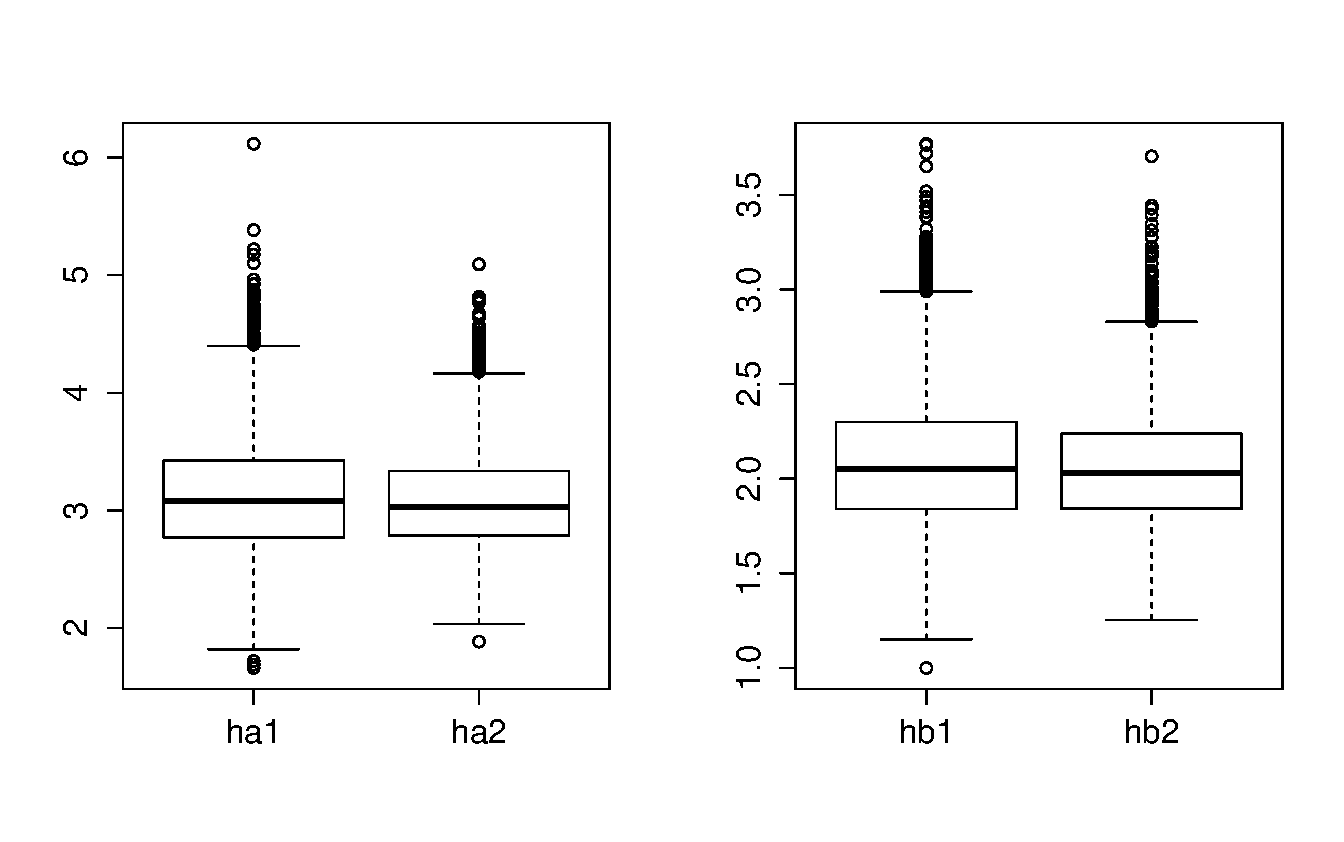
\includegraphics[width=0.8\textwidth]{boxplot1}\\
  \caption{Boxplot: paramètres $\alpha=3$, $\beta=2$, $n=100$, $5000$ réplications indépendantes}
\end{figure}
\end{frame}




\begin{frame}
\frametitle{Distribution asymptotique - $n=500$}
\begin{figure}
  \centering
  % Requires \usepackage{graphicx}
  \includegraphics[width=0.8\textwidth]{distribution500}\\
  \caption{Boxplot: paramètres $\alpha=3$, $\beta=2$, $n=500$, distribution asymptotique, bootstrap et bootstrap paramétrique}
\end{figure}
\end{frame}

\begin{frame}
\frametitle{Distribution asymptotique - $n=20$}
\begin{figure}
  \centering
  % Requires \usepackage{graphicx}
  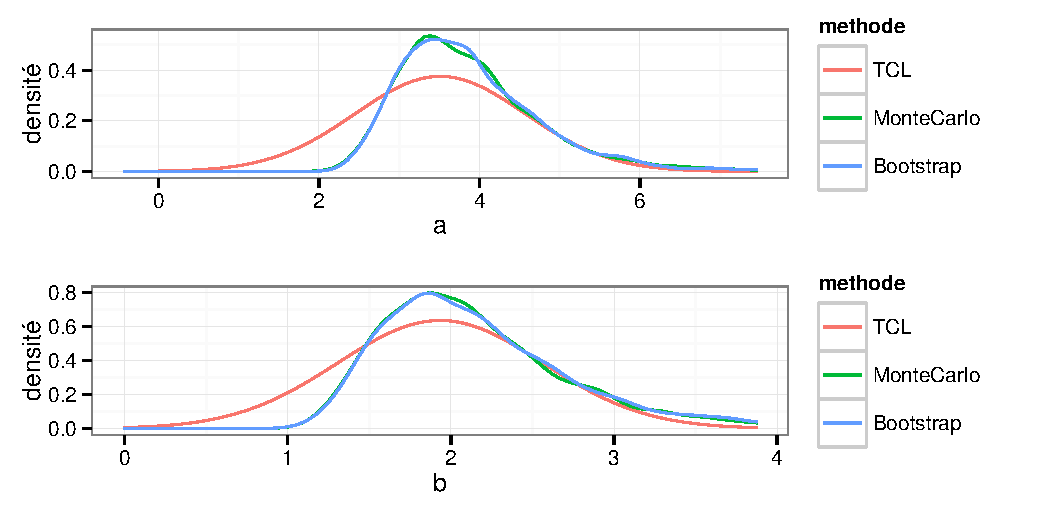
\includegraphics[width=0.8\textwidth]{distribution20}\\
  \caption{Boxplot: paramètres $\alpha=3$, $\beta=2$, $n=500$, distribution asymptotique, bootstrap et bootstrap paramétrique}
\end{figure}

\end{frame}


\end{document} 